
\documentclass[border=5pt]{standalone}
\usepackage{pgfplots}
\pgfplotsset{compat=1.18}
\usepackage{amsmath}
\begin{document}
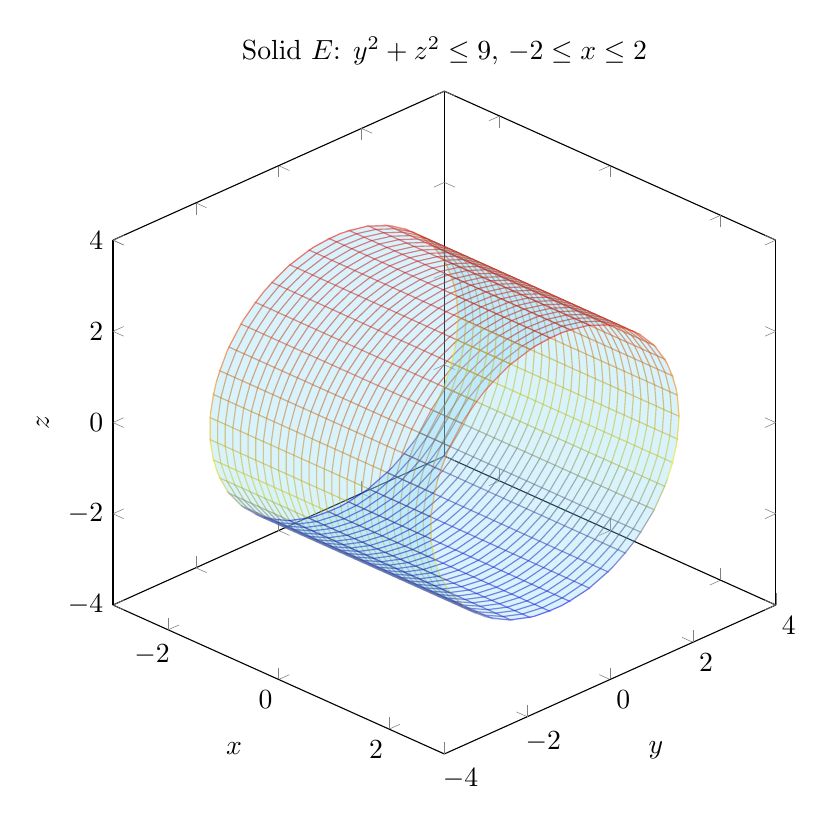
\begin{tikzpicture}
\begin{axis}[
    width=10cm, height=10cm,
    xlabel={$x$}, ylabel={$y$}, zlabel={$z$},
    xmin=-3, xmax=3, ymin=-4, ymax=4, zmin=-4, zmax=4,
    view={45}{30},
    title={Solid $E$: $y^2+z^2 \leq 9$, $-2 \leq x \leq 2$},
]
% Cylinder lateral surface
\addplot3[
    surf, opacity=0.3, fill=cyan!50,
    domain=-2:2, y domain=0:2*pi,
    samples=30, samples y=40,
] (x, {3*cos(deg(y))}, {3*sin(deg(y))});
% End cap at x=-2
\addplot3[
    surf, opacity=0.4, fill=red!60,
    domain=0:2*pi, y domain=0:2*pi,
    samples=30, samples y=1,
] (-2, {3*cos(deg(x))}, {3*sin(deg(x))});
% End cap at x=2
\addplot3[
    surf, opacity=0.4, fill=green!60,
    domain=0:2*pi, y domain=0:2*pi,
    samples=30, samples y=1,
] (2, {3*cos(deg(x))}, {3*sin(deg(x))});
\end{axis}
\end{tikzpicture}

\vspace{1em}
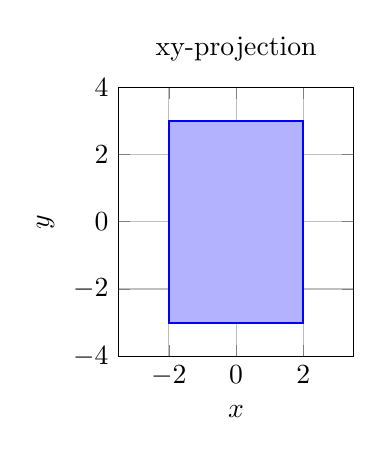
\begin{tikzpicture}
% Projection on xy-plane
\begin{axis}[
    width=5cm, height=5cm,
    xlabel={$x$}, ylabel={$y$},
    xmin=-3.5, xmax=3.5, ymin=-4, ymax=4,
    axis equal image, grid=both,
    title={xy-projection},
]
\fill[blue!30] (axis cs:-2,-3) rectangle (axis cs:2,3);
\draw[blue, thick] (axis cs:-2,-3) rectangle (axis cs:2,3);
\end{axis}
\end{tikzpicture}
\hspace{1em}
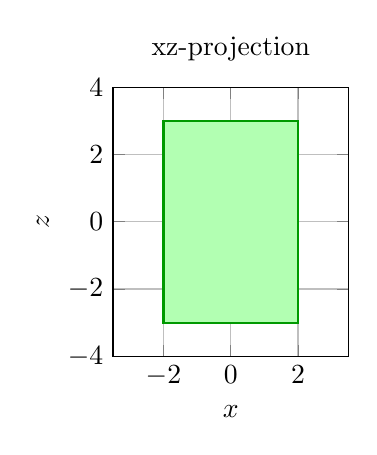
\begin{tikzpicture}
% Projection on xz-plane
\begin{axis}[
    width=5cm, height=5cm,
    xlabel={$x$}, ylabel={$z$},
    xmin=-3.5, xmax=3.5, ymin=-4, ymax=4,
    axis equal image, grid=both,
    title={xz-projection},
]
\fill[green!30] (axis cs:-2,-3) rectangle (axis cs:2,3);
\draw[green!60!black, thick] (axis cs:-2,-3) rectangle (axis cs:2,3);
\end{axis}
\end{tikzpicture}
\hspace{1em}
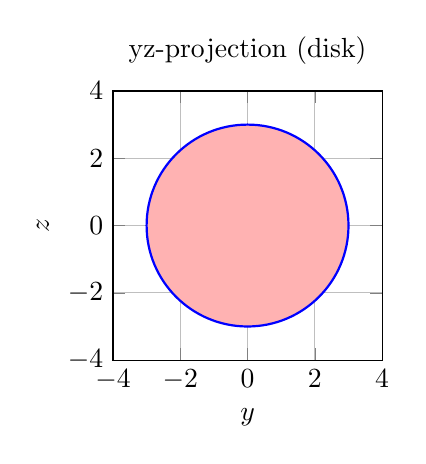
\begin{tikzpicture}
% Projection on yz-plane (disk)
\begin{axis}[
    width=5cm, height=5cm,
    xlabel={$y$}, ylabel={$z$},
    xmin=-4, xmax=4, ymin=-4, ymax=4,
    axis equal image, grid=both,
    title={yz-projection (disk)},
]
\fill[red!30] (axis cs:0,0) circle [radius=3];
\draw[blue, thick] (axis cs:0,0) circle [radius=3];
\end{axis}
\end{tikzpicture}
\end{document}
